\begin{titlepage}
\begin{center}

{\small Київський національний університет  імені Тараса Шевченка}

{\small фізичний факультет}


\vspace*{2cm}
{\scshape\bfseries\Large О.Я.~ОЛІХ}

\vspace*{1cm}
{\scshape\bfseries\huge методи дослідження дефектів}

\vspace*{0.5cm}
методичний посібник для студентів фізичного факультету

\end{center}
%
\vspace*{2cm}
\begin{figure}[h]\center
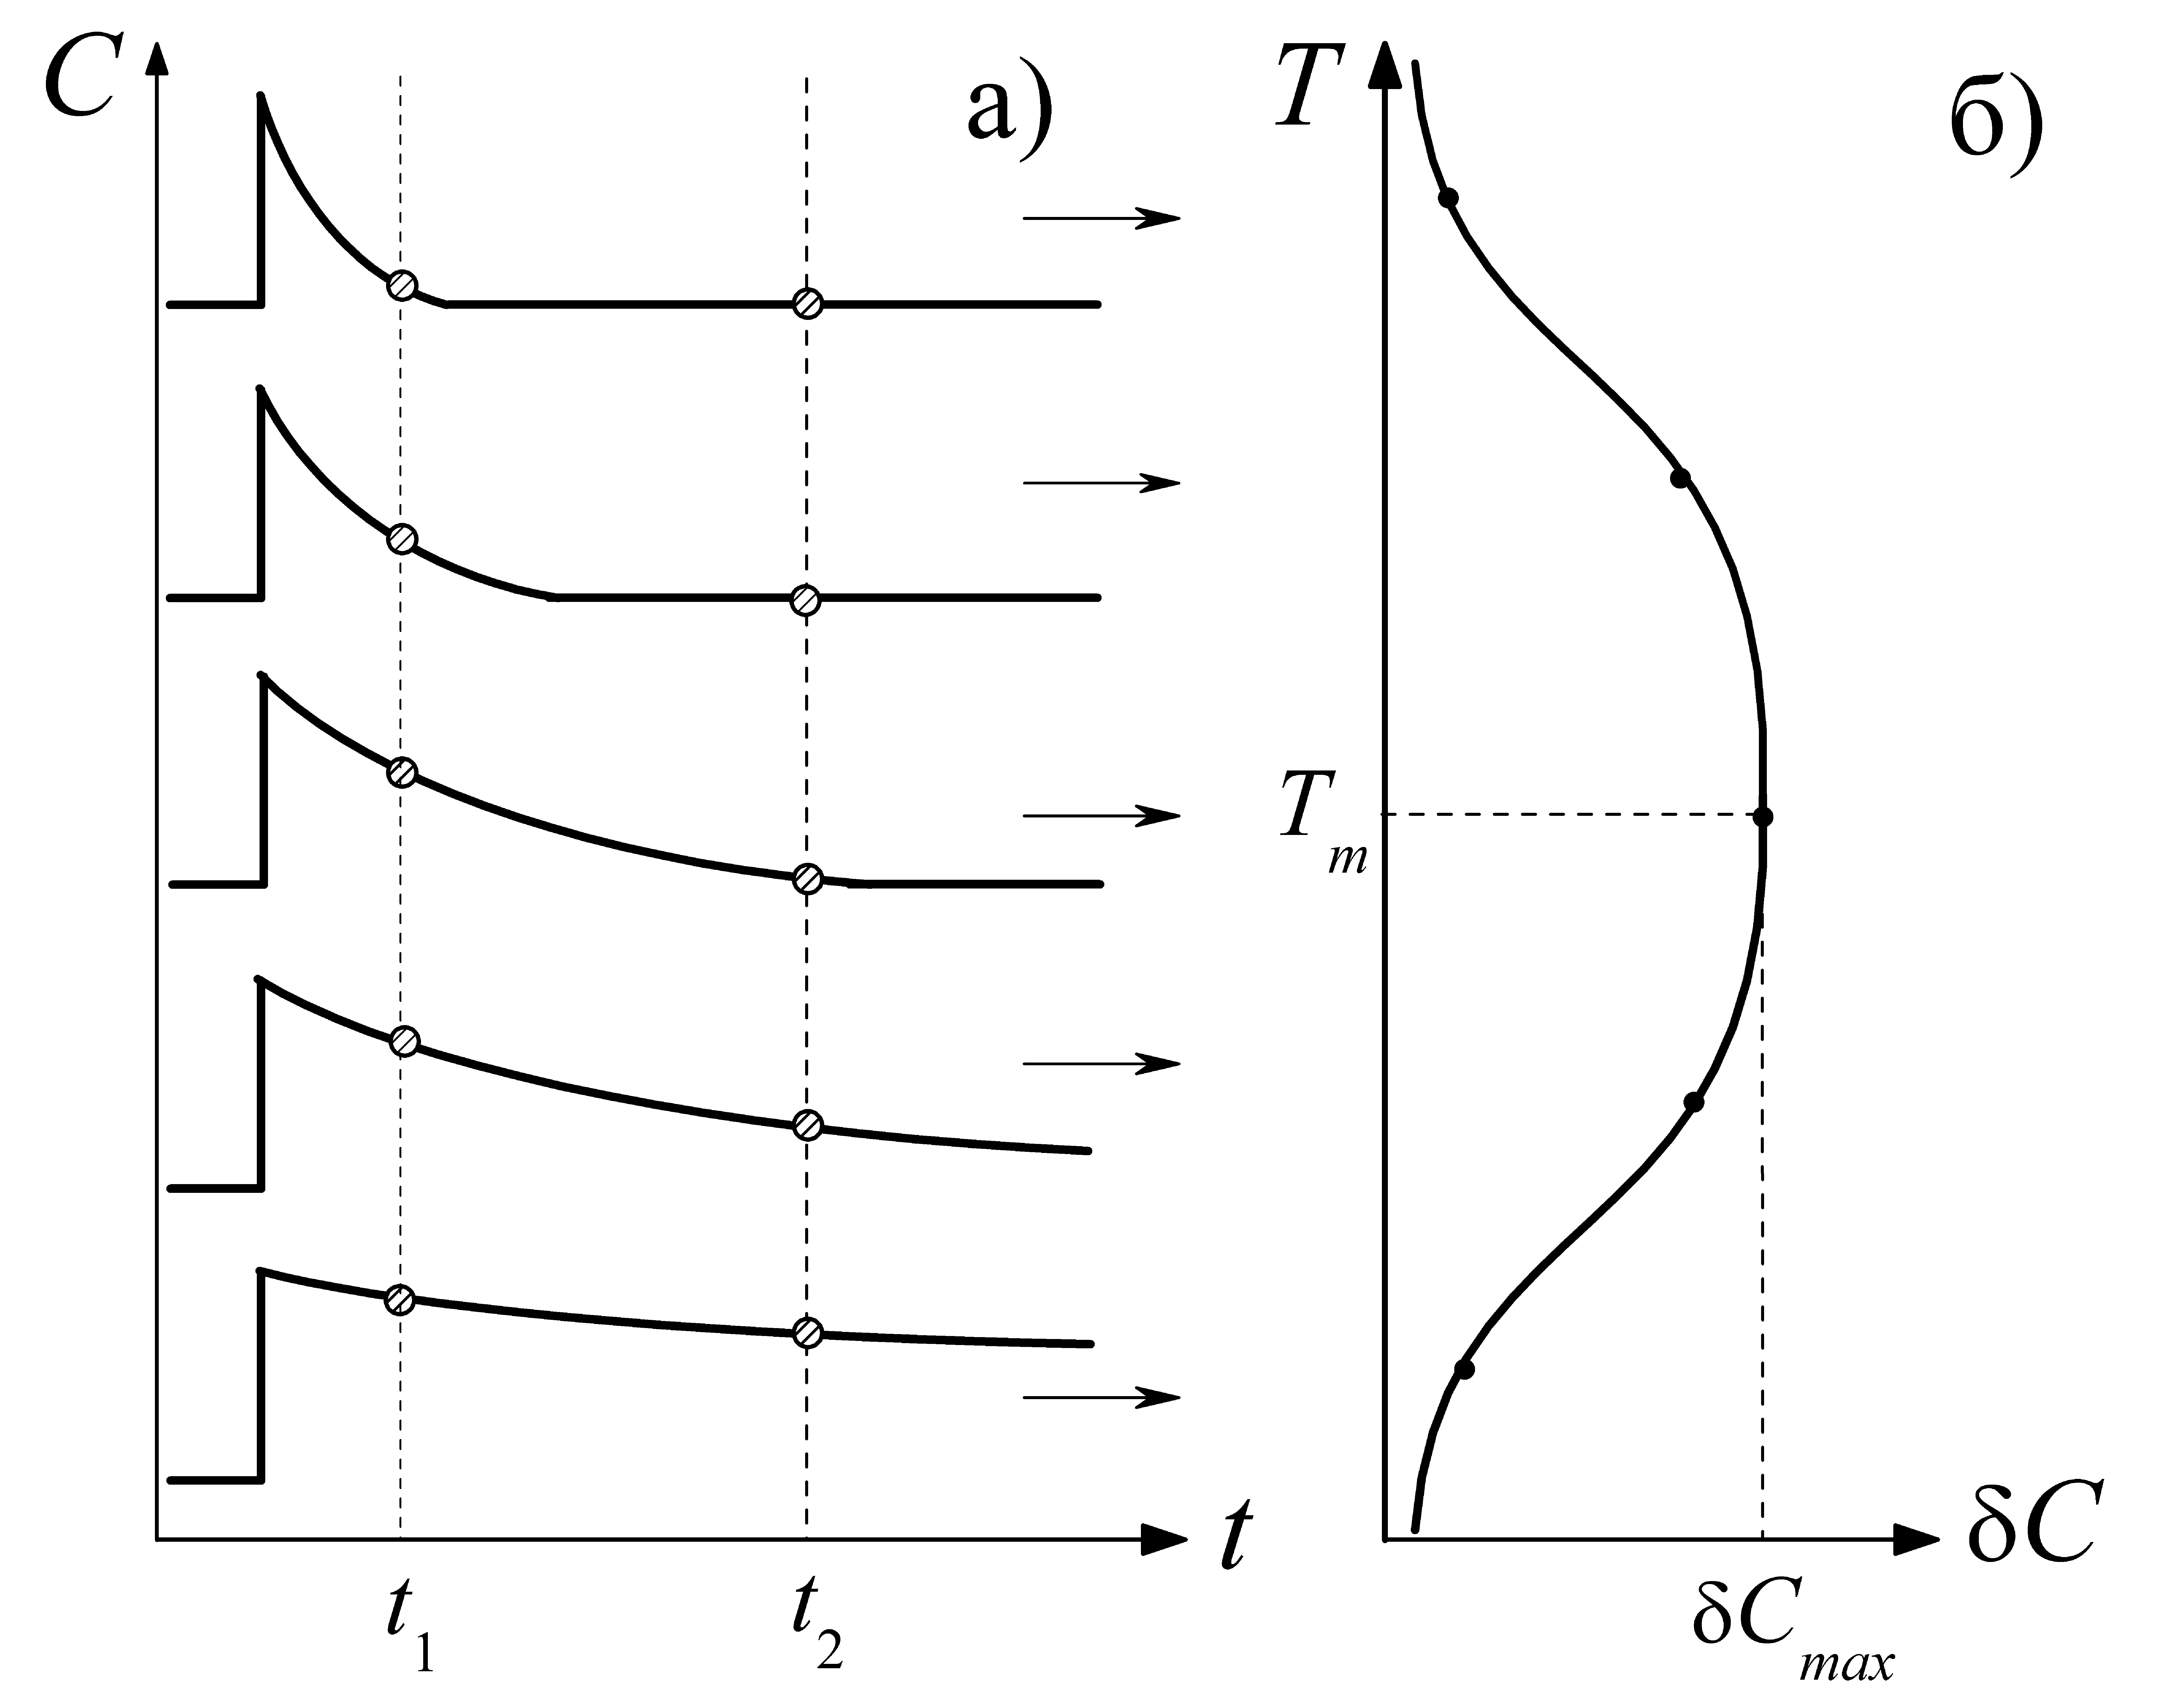
\includegraphics[width=0.8\textwidth]{Fig2_3}
\end{figure}
%
%
\begin{center}

{\scshape\bfseries Київ -- 2020}
\end{center}
\end{titlepage}
Б

УДК 004.7; 004.057.4.

\begin{center}

 \vspace{0.04\textheight}
 Рецензенти:
\end{center}
%\vspace{0.5cm}

%\emph{С.В.~Кондратенко}, д-р. фіз.-мат. н., проф.
%
%\emph{О.О.~Коротченков}, д-р. фіз.-мат. н., проф.

\vspace{1cm}
Рекомендовано до друку вченою радою фізичного факультету
Київського національного університету імені Тараса Шевченка
%(протокол №10 від 18 квітня 2020 року)



\vspace{1cm}
\textbf{Оліх О.Я.}

Методи дослідження дефектів. Методичний посібник для студентів фізичного факультету. --- К.:2020.
%Іл.~236, табл.~51.

\vspace{1cm}
У посібнику розглянуто як основні електричні параметри дефектів,
так і представлено методи їхнього дослідження.
Зокрема розглянуто методи перехідної спектроскопії, 
позитронно--анігіляційної спектроскопії,
термостимульованих струмів,
магніто--резонансні
та диференційних коефіцієнтів вольт--амперних характеристик.
Призначений для студентів фізичного факультету, а також
може бути корисний для науковців  та  здобувачів  ступеня  доктор  філософії  
відповідних спеціальностей.